
This section provides a formal model of the problem described with Alloy modeling language. 
The model considers the most important constraints. In addition to the model there are some 
possible worlds meant to clarify some critical aspects.


\subsection{Alloy model}
\lstinputlisting[language=alloy]{alloy_model.als}

\subsection{First World}
In the first world (Figure \ref{fig:world1}) the focus is on the \textsl{registration} of two farmers. 
Since we assume that they use the application for the first time, the only information present 
are the ones required for the registration. Email and username are unique. On the contrary password and 
surname can be the same for different farmers. Another thing to notice is that email, username, surname and password do not 
exist without an associated user. 
Given that each farmer is associated to a farm, creating a world with two farmers, automatically considers
the same amount of different farm as well. The number of policy makers is zero to 
highlight the fact that farmers do not depend directly with policy makers.



\subsection{Second World}
The second world showed in Figure \ref{fig:world2} focuses on a single farm with \textsl{multiple evaluations}. 
Therefore it is considered a farm, with its owner and all their characteristics. 
Every evaluation made on the farm has a different date, more precisely it does not 
have the same month, and a different messageContent. They are written by different policy 
makers but the most important thing to notice is that the receiver of the evaluation 
is the same owner of the farm that has the evaluation.


\subsection{Third World}
The third world (Figure \ref{fig:world3}) highlights the possibility 
of the farmers to communicate to each other through the forum. The farmer can send messages and fill in a report with a production he made in his 
farm in a specific date. Each message sent in the forum has exactly 
one sender (a farmer only). The system also verifies that the sender can write 
one message at a time. 
The forum is unique but it can be empty (look at world 1) if nobody has sent any message yet. 
On the other side each production submitted in a day must be of different types. As a matter of fact the form 
has the field ‘quantity’ used to specify the amount so it is not necessary to generate a production for each harvest.

\begin{sidewaysfigure}
    \begin{center}
          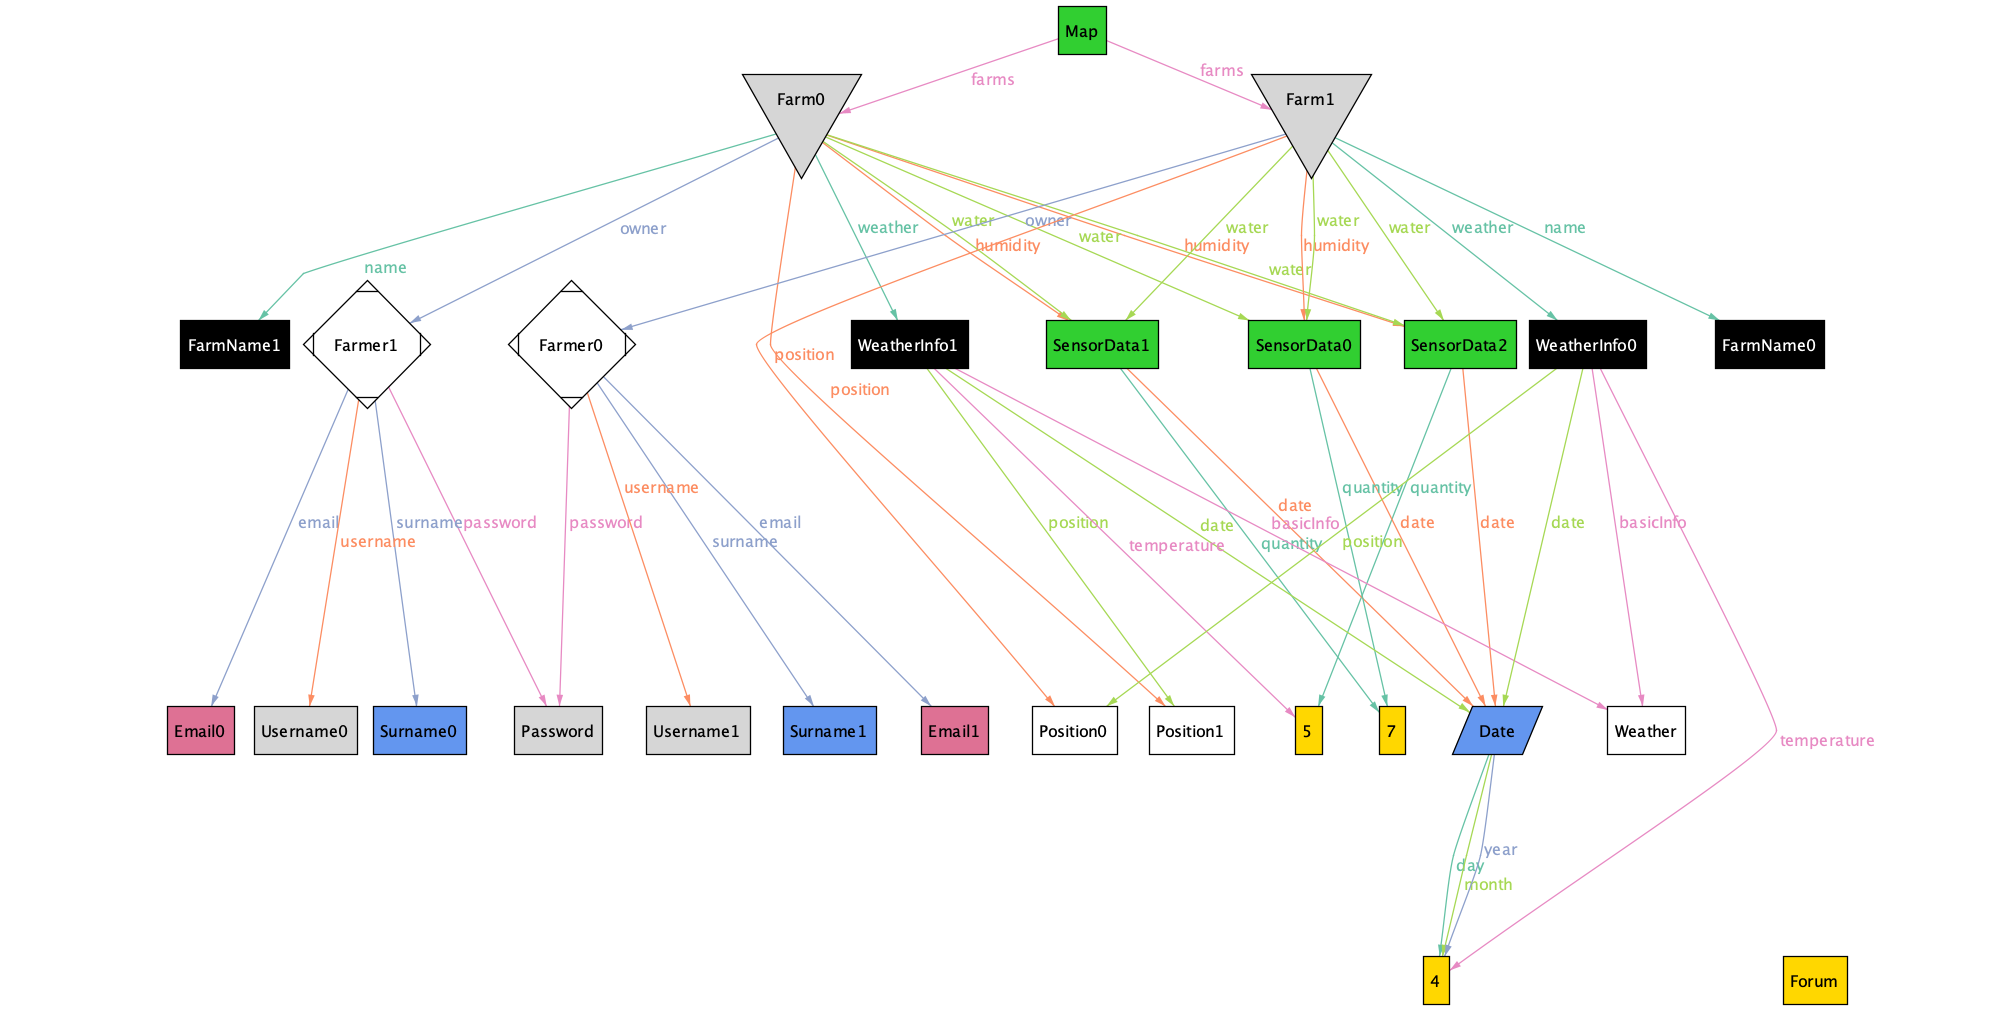
\includegraphics[width=1.2\textwidth]{alloy/world1.png}
          \caption{FirstWorld}
        \label{fig:world1}
    \end{center}
\end{sidewaysfigure}


\begin{sidewaysfigure}
    \begin{center}
          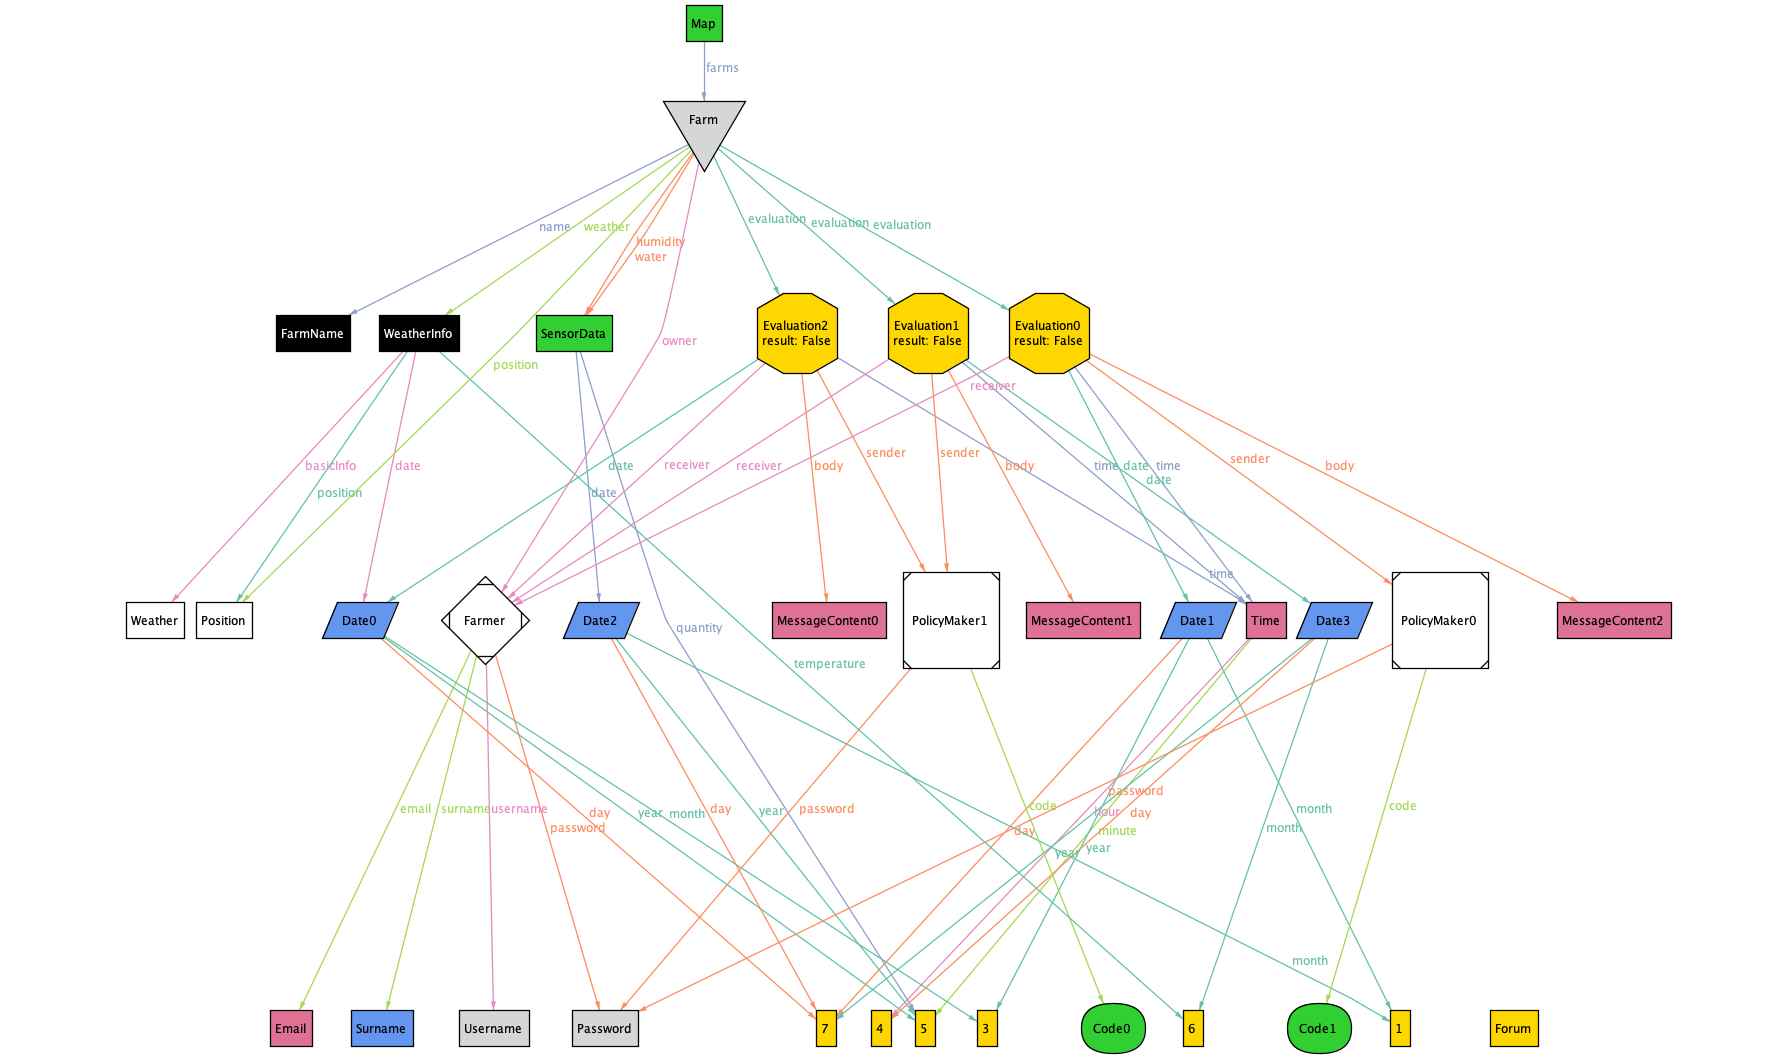
\includegraphics[width=1.2\textwidth]{alloy/world2.png}
          \caption{Second World}
        \label{fig:world2}
    \end{center}
\end{sidewaysfigure}

\begin{sidewaysfigure}
    \begin{center}
          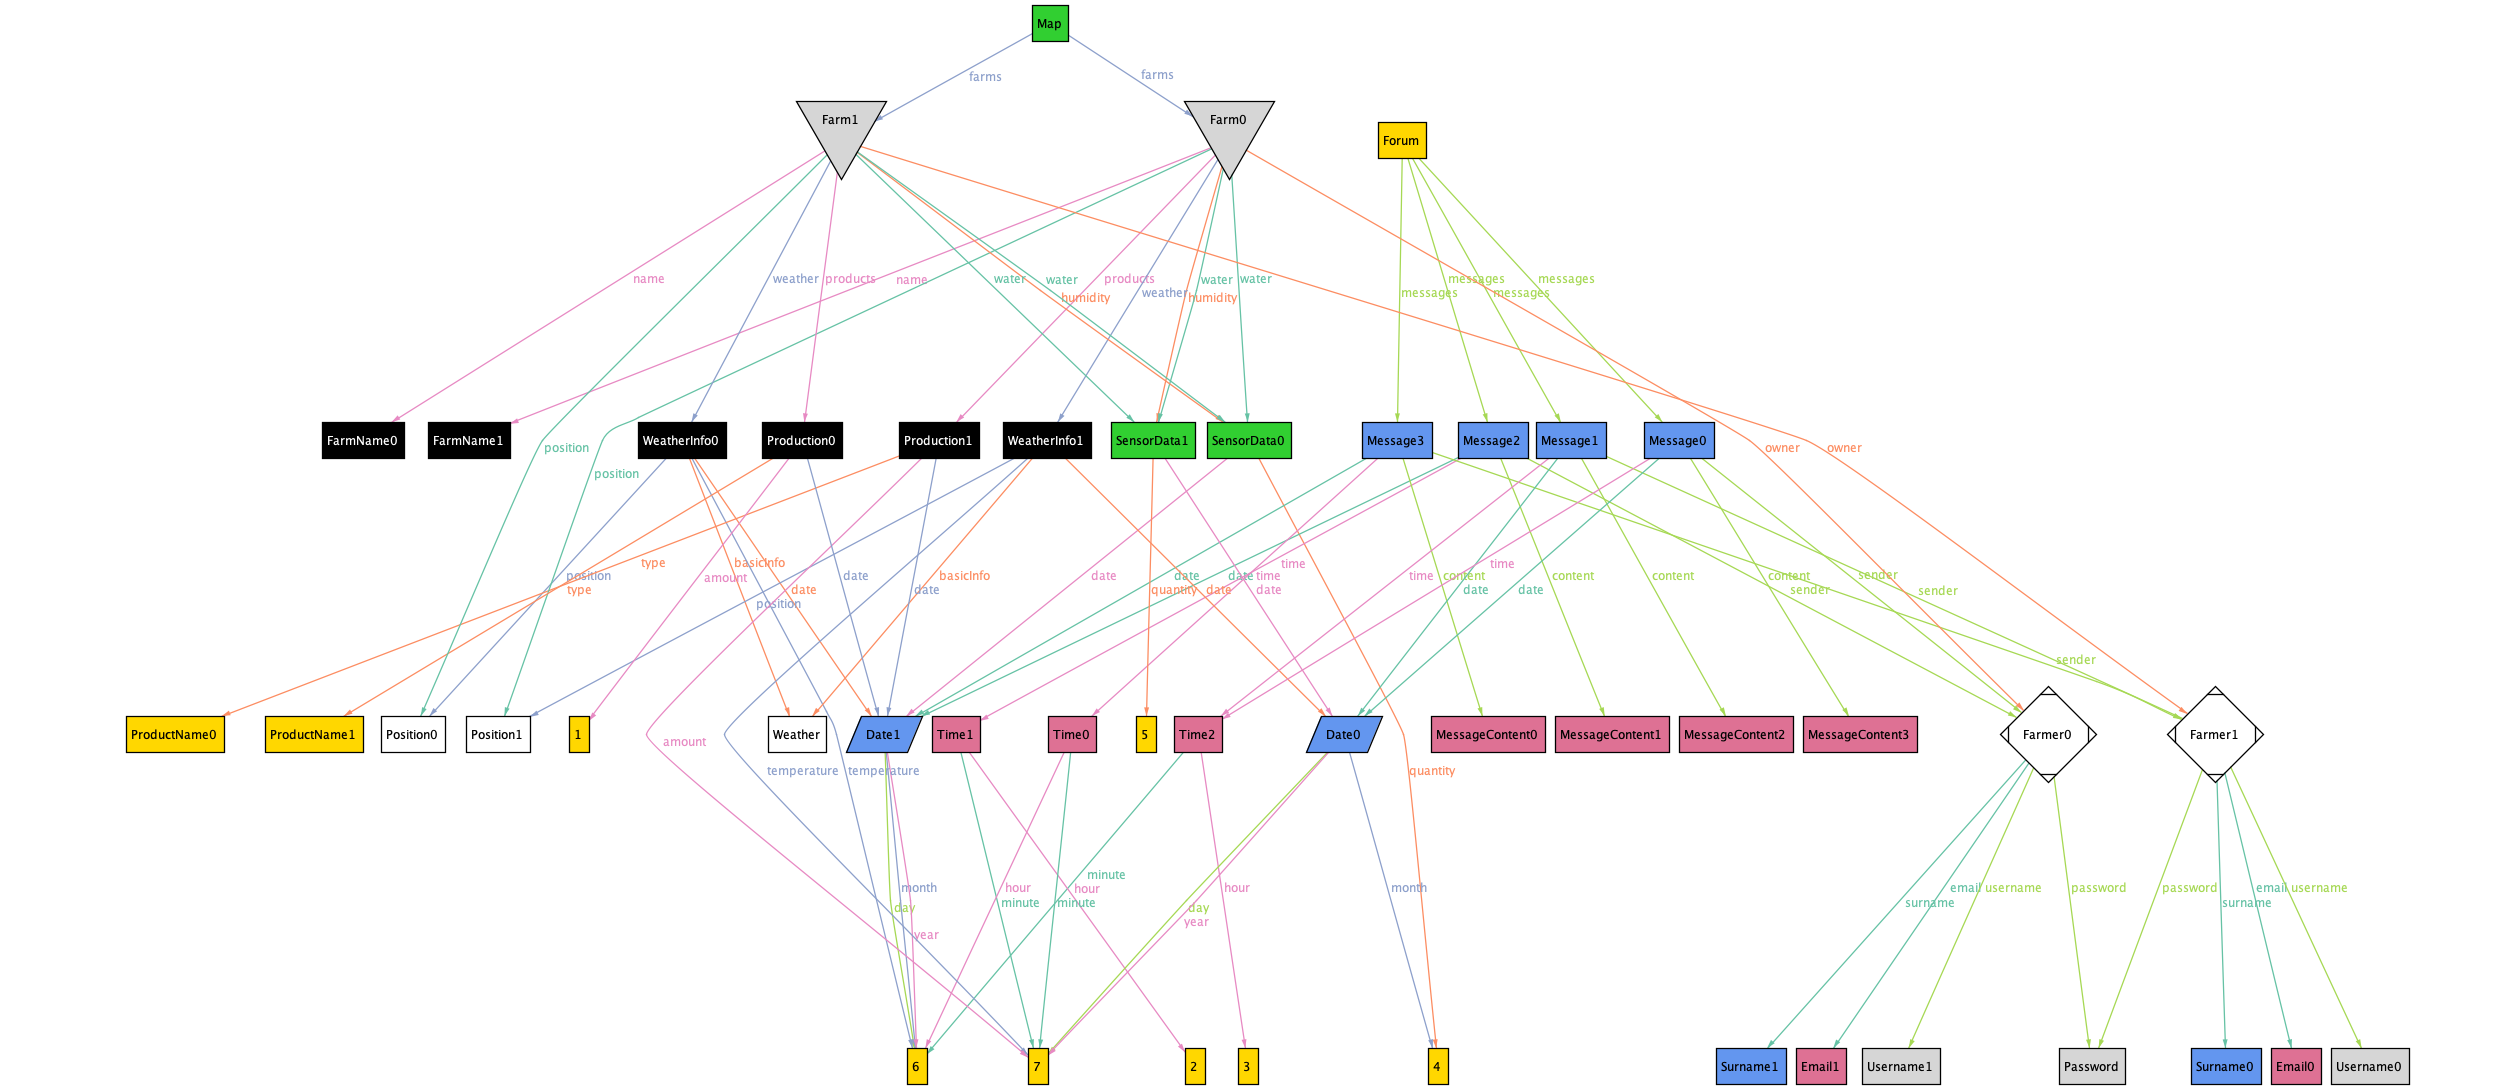
\includegraphics[width=1.2\textwidth]{alloy/world3.png}
          \caption{Third World}
        \label{fig:world3}
    \end{center}
\end{sidewaysfigure}

